\section*{I/O Devices (allows information to persist; RAM is volatile)}
\begin{minipage}{.5\linewidth}
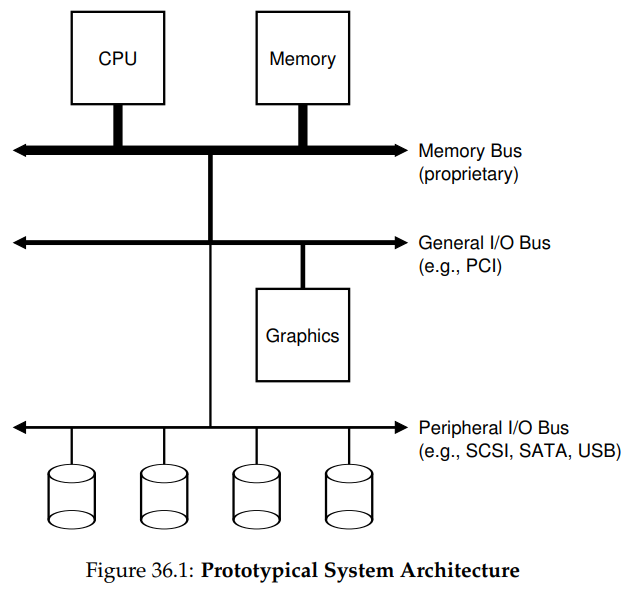
\includegraphics[width=\linewidth]{imgs/prototypical_sys_arch}
\end{minipage}
\begin{minipage}{.5\linewidth}
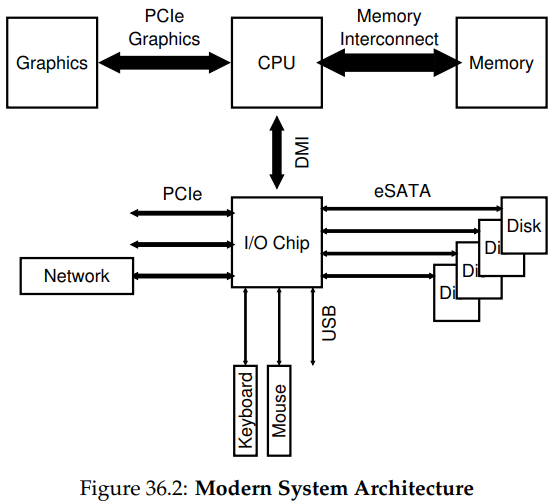
\includegraphics[width=\linewidth]{imgs/modern_sys_arch}
\end{minipage}
\begin{minipage}{.5\linewidth}
  \flushleft
  \begin{itemize}
  \item The faster a bus is, the shorter it must be $\to$ high-performance memory bus doesn't have much room for many devices
  \item components that demand high performance (such as graphics card) placed nearer CPU
  \item lower performance components are further away
  \end{itemize}
\end{minipage}
\begin{minipage}{.5\linewidth}
  \flushleft
  \begin{itemize}
  \item modern sys use specialized chipsets and faster point-to-point inter-conn to $\uparrow$ performance; USB (Universal Serial Bus) is used for low performance devices
  \item OS handles device management (and access); OS exposes uniform interface to applications
  \item IO is interrupt driven
  \end{itemize}
\end{minipage}
\begin{minipage}{.65\linewidth}
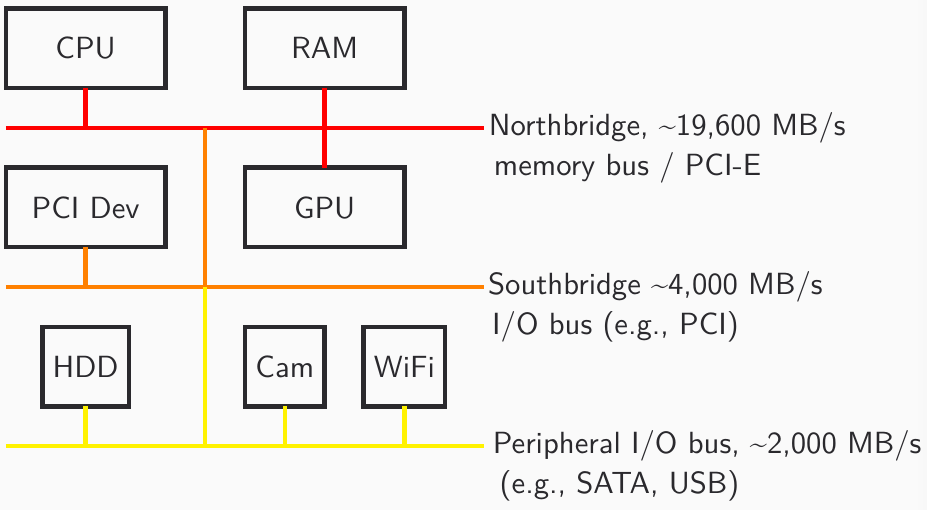
\includegraphics[width=\linewidth]{imgs/otherio}
\end{minipage}
\begin{minipage}{.35\linewidth}
  \flushleft
  \begin{itemize}
  \item Northbridge, aka memory controller hub
  \item Southbrigge, aka I/O Controller Hub (Intel) or Fusion Controller Hub (AMD)
  \item southbridge connected to CPU through northbridge which has a direct connection
  \end{itemize}
\end{minipage}
\section*{Canonical Devices (an abstraction with 2 components)}
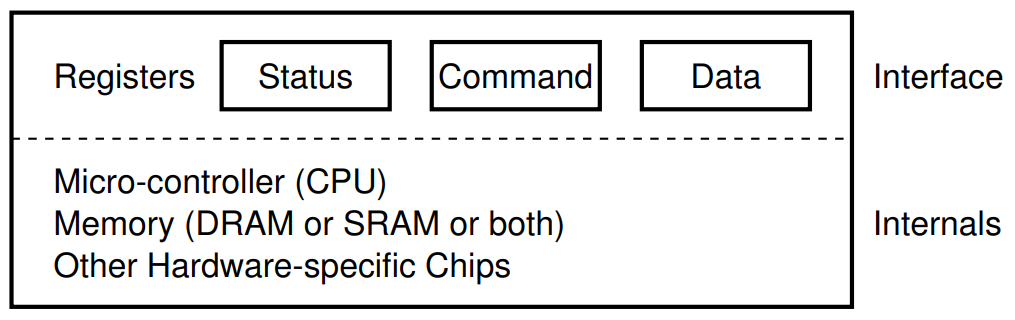
\includegraphics[width=\linewidth]{imgs/canonical_dev}
\begin{itemize}
\item \textbf{status} register to be read to see the current status of the device
\item \textbf{command} register to tell the device to perform a certain task
\item \textbf{data} register pass data to the device, or get data from
the device
\end{itemize}
\begin{enumerate}
\item \textbf{hardware interface} presents to the rest of the system. Hardware must present some kind of interface that allows the system
software to control its operation. Thus, all devices have some specified
interface and protocol for typical interaction
\item \textbf{internal structure}, implementation specific and responsible for implementing the abstraction the device presents to the system
  \begin{itemize}
  \item Very simple devices will have one/a few hardware chips
  \item more complex devices will include a simple CPU, some general purpose
memory, and other device-specific chips, e.g modern RAID controllers might consist of hundreds of thousands of lines of firmware (i.e. software within a hardware device)  to impl. its functionality
  \end{itemize}
\end{enumerate}
\section*{Canonical Protocol (4 steps, simple yet inefficient)}
\begin{enumerate}
\item OS waits until the device ready to receive a command by repeatedly reading the status register (\textbf{polling} the device)
\item OS sends some data down to data register
  \begin{itemize}
  \item multiple writes to transfer a disk block (say 4KB) to the device
  \item if main CPU involved (as in this case) $\to$ \textbf{programmed I/O} (PIO)
  \end{itemize}
\item OS writes a command to command register $\to$ implicitly tell the device that data is present and device should begin working on the command
\item OS waits for the device to finish by again polling it in a loop, waiting to see if it is finished (return code for success/error)
\end{enumerate}
\begin{lstlisting}[language=c]
While (STATUS == BUSY)
    ; // wait until device is not busy
Write data to DATA register // set up everything before any cmd exec
Write command to COMMAND register
    (starts the device and executes the command)
While (STATUS == BUSY)
    ; // wait until device is done with your request
\end{lstlisting}
\section*{Lowering CPU Overhead with Interrupts}
\begin{minipage}{.5\linewidth}
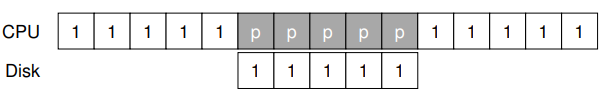
\includegraphics[width=\linewidth]{imgs/iopolling}
\end{minipage}
\begin{minipage}{.5\linewidth}
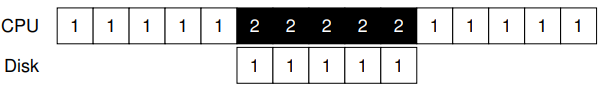
\includegraphics[width=\linewidth]{imgs/iointerrupt}
\end{minipage}
\begin{minipage}{.5\linewidth}
  \flushleft
  \begin{enumerate}
  \item $P_1$ runs on CPU for some time (repeated \texttt{1} on CPU line)
  \item then issues I/O request to disk to read some data
  \item OS spins, polling status of device repeatedly until I/O completes
  \item disk serves req; $P_1$ can run again
  \end{enumerate}
\end{minipage}
\begin{minipage}{.5\linewidth}
  \flushleft
  \begin{enumerate}
  \item OS runs $P_2$ on CPU while disk services $P_1$'s request
  \item When disk request is done, an interrupt occurs
  \item OS wakes up $P_1$, runs it again
  \item \mb{both} CPU and disk get properly utilized during the middle
  \end{enumerate}
\end{minipage}
\begin{tcolorbox}[left=0mm, top=1mm, right=0mm, rightlower=0mm, bottom=1mm,
  title= Interrupts \mr{NOT always} better than polling,
  halign title=center]
  Although interrupts allow for overlap of computation and I/O, they only
  really \mb{make sense for slow devices}. Otherwise, the cost of interrupt handling and context switching may outweigh the benefits interrupts provide.  If a device performs its tasks \emph{very quickly}: the 1st poll usually finds the device done with task. Using an interrupt in this case will actually \emph{slow down} the system: switching to another process, handling the interrupt, and switching back to the issuing process is expensive.

  There are also cases where a flood of interrupts may overload a system and lead it to \textbf{livelock}; in such cases, polling provides more control to the OS in its scheduling and thus is again useful.
\end{tcolorbox}
\begin{itemize}
\item if a device is fast, best to poll; if it's slow, best to interrupt (overlap)
\item If device speed is unknown (sometimes fast, sometimes slow), best to \textbf{hybrid}: polls for a short while and if device not yet finished, interrupts
\item This \textbf{two-phased} approach may achieve the best of both worlds
\end{itemize}
In networks, when a huge stream of incoming packets each generate an interrupt, OS may \textbf{livelock}: find itself only processing interrupts and never running a user-level process and actually servicing requests
\begin{itemize}
\item a web server with a load burst $\because$ it became top-ranked on hacker news
\item In this case, it's better to occasionally poll to better control what's happening in system and allow server to fulfill some requests before going back to the device to check for more packet arrivals
\end{itemize}
Another interrupt-based optimization is \textbf{coalescing}:
\begin{itemize}
\item a device first waits for a bit before delivering its interrupt to CPU
\item While waiting, other requests may soon complete $\to$ multiple interrupts can be coalesced into a single delivery $\to$ lowering overhead
\item yet waiting too long $\to$ request latency $\uparrow$: common trade-off in systems
\end{itemize}
\section*{More Efficient Data Movement With DMA}
\begin{minipage}{.5\linewidth}
  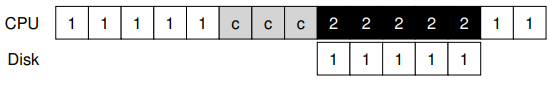
\includegraphics[width=\linewidth]{imgs/dma1}
\end{minipage}
\begin{minipage}{.5\linewidth}
  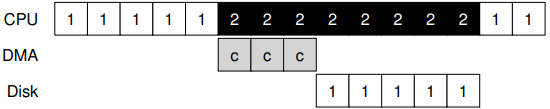
\includegraphics[width=\linewidth]{imgs/dma2}
\end{minipage}
\begin{minipage}{.5\linewidth}
  \flushleft
   overburdened OS wastes cycles
  \begin{enumerate}
  \item $P_1$ runs \& wants to write to disk
  \item $P_1$ init I/O and copy data from memory to device explicitly, one word at a time (\texttt{c} in diagram)
  \item when done, I/O starts on disk
  \item CPU finally works on sth else
  \end{enumerate}
\end{minipage}
\begin{minipage}{.5\linewidth}
  \flushleft
  \begin{enumerate}
  \item OS tells DMA engine where data lives in memory (pass a pointer)
  \item OS done with trans; proceeds with other work
  \item DMA works on data trans; when done, raises interrupt to notify OS
  \end{enumerate}
\end{minipage}
\begin{tcolorbox}[left=0mm, top=1mm, right=0mm, rightlower=0mm, bottom=1mm,
  title= DMA Attack,
  halign title=center]
  A drawback of DMA (from security viewpoint): it bypasses the kernel -- no oversight on the memory access. This can lead to system exploitation through externally connected devices through, e.g., Thunderbolt, USB 4.0, FireWire, etc.
\end{tcolorbox}

\section*{2 Methods of Device Interaction (OS communicates with the device)}
\begin{enumerate}
\item \textbf{I/O ports} (IBM) with special instructions for OS to send/recv data
  \begin{itemize}
  \item on x86 \texttt{in} and \texttt{out} ixs use \mo{port} that names device to send/recv data
  \item ixs are \mb{privileged} $\to$ \emph{only} OS can communicate with devices
  \end{itemize}
\item \textbf{Memory Mapped IO}  hardware makes device registers
  available as if they were memory locations
  \begin{itemize}
  \item OS issues load (read) or store (write) to access particular reg (addr)
  \item hardware then routes load/store to device instead of main memory
  \end{itemize}
\end{enumerate}
\begin{itemize}
\item memory-mapped approach is nice $\because$ no new ixs needed to support it
\item \mb{both} approaches still in use;  architectures support both
\item Differences are a matter of choice and preference
\end{itemize}
\section*{Device Driver to help devices fit into OS}
\begin{minipage}{\linewidth}
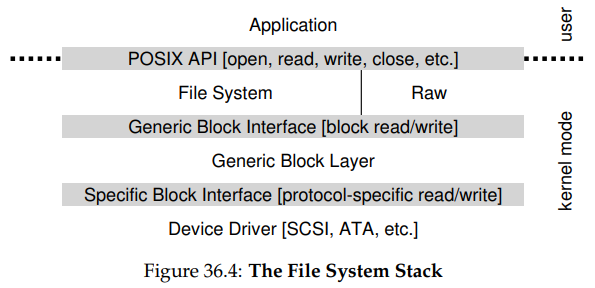
\includegraphics[width=\linewidth,height=3.8cm]{imgs/filesys_stack}
\flushleft
Diagram also shows a \textbf{raw interface} to devices that enables special apps (e.g.\textbf{file-system checker} or \textbf{disk defragmentation} tool) to directly read and write blocks without using file abstraction. Most sys provide such interface to support low-level storage management apps.
\end{minipage}
\begin{itemize}
\item goal: keep devices as general as possible so OS works with most devs
\item challenges: different devices have \emph{different} protocols
\item drivers: specialty pieces of code for particular device (\textbf{encapsulation}): \mo{low} end comm. with device; \mo{high} end exposes generic interface to OS
\item requirement: well-designed interface/API: 1. trade-off between versatility and over-specialization; 2. device class complexity $\to$ OS ends with layers of APIs (70\%+ code for device drivers in Linux Kernel)
\item Downside: device with rich features cannot use all of them $\because$ it must present a generic interface to kernel. In Linux, SCSI devices have very rich error reporting; but other block devices (ATA/IDE) have much simpler error handling so all higher levels of software just recv a generic \texttt{EIO} (generic IO error code); any extra detail of SCSI thus lost
\end{itemize}
